\begin{enumerate}
\item Открыть Vivado проект из lab2-1
\item Добавить в проект файл тестбенча. Для этого
а) Под закладкой \emph{Project Manager} нажать \emph{Add Souces}, выбрать пункт \emph{Add or Create Simulation Sources} (см. рис. \ref{add_sim_src_1}).

% \begin{figure}[ht]
\begin{figure}
\centering
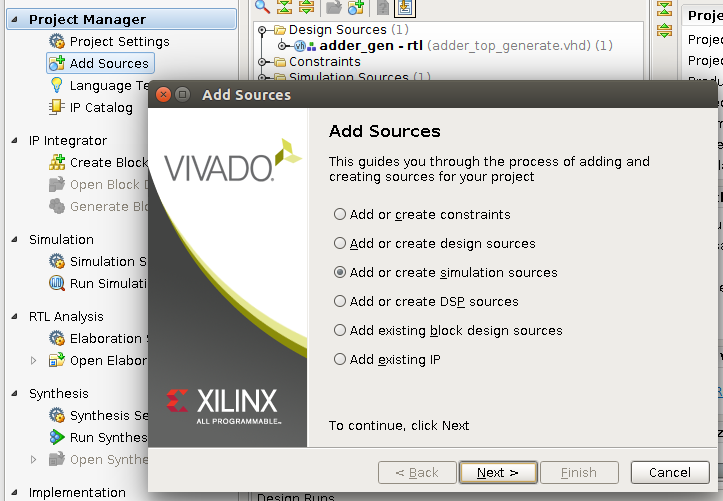
\includegraphics[width=1.2\textwidth]{03-vhdl_modeling/fig/add_sim_src_1.png}
\caption{Выбор типа исходных файлов}
\label{add_sim_src_1}
\end{figure}

б) В следующем окне нажать \emph{Add Files} и выбрать файл \emph{02-vhdl\_basics/lab2-1/src/adder\_tb\_simple.vhd}. После выбора файла окно должно выглядеть как на рис. \ref{add_sim_src_2}. Нажать кнопку \emph{Finish}. В итоге в Vivado окошко \emph{Sources} должно выглядеть следующим образом (рис. \ref{add_sim_src_3}).

% \begin{figure}[ht]
\begin{figure}
\centering
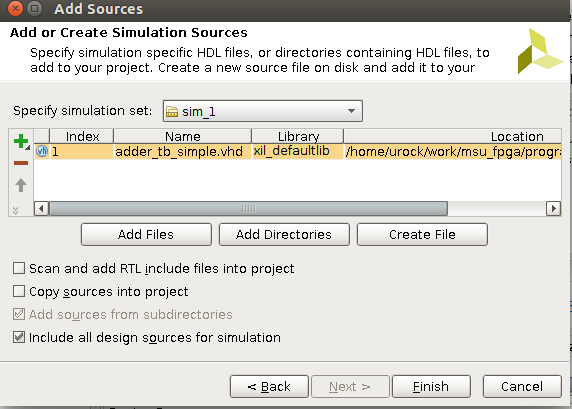
\includegraphics[width=1.2\textwidth]{03-vhdl_modeling/fig/add_sim_src_2.png}
\caption{Выбор файла тестбенча}
\label{add_sim_src_2}
\end{figure}

\begin{figure}
\centering
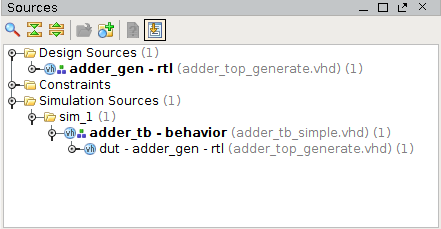
\includegraphics[width=0.8\textwidth]{03-vhdl_modeling/fig/add_sim_src_3.png}
\caption{Окно Sources после добавления файла тестбенча}
\label{add_sim_src_3}
\end{figure}


TODO:
1. Запретить разбивать листинги на части 
2. Научиться настраивать ширину поля листинга


\item Открыть окно \emph{Simulation Settings} и настроить полное время моделирования схемы (см. рис. \ref{sim-setting}). Оставить параметр \emph{xsim.simulate.runtime} равным 1000ns.

\begin{figure}
\centering
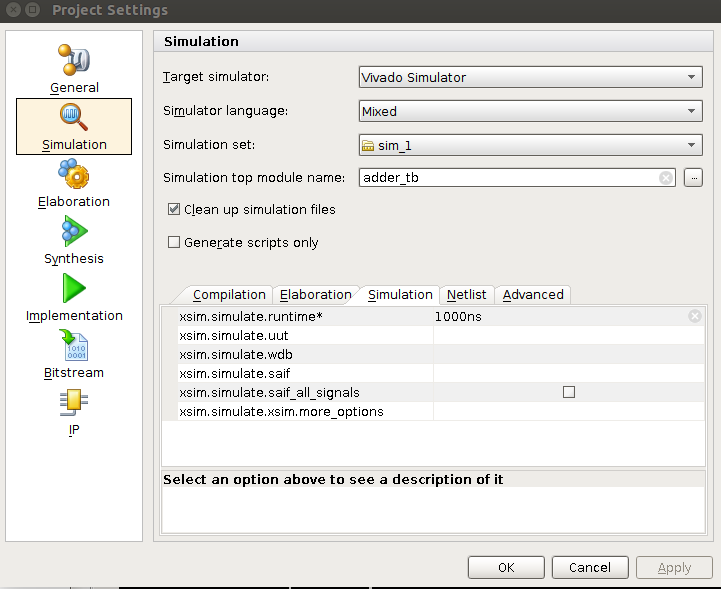
\includegraphics[width=1.2\textwidth]{03-vhdl_modeling/fig/sim-settings.png}
\caption{Окно параметров моделирования}
\label{sim-setting}
\end{figure}


\item Запустить симуляцию. Для этого выбрать \emph{Simulation->Run Simulation->Run  Behavioral Simulation}. Откроется три окна. В первом (\emph{Scopes}) можно видеть иерархию VHDL модулей. Во втором (\emph{Objects}) отображается список сигналов этого модуля. В окне \emph{Scopes} можно выбрать любой модуль иерархии, а потом в окне \emph{Objects} выбрать интересующие сигналы и добавить их на вейформу, нажав правой кнопкой мыши по выбранным сигналам и выбрав \emph{Add to Wave Window}. В третьем окне открывается времянные диаграммы (вейформы) сигналов (cм. рис. \ref{tb-wave}). Чтобы в окне вейформ было показано полное время симуляции, надо нажать правой кнопкой и выбрать \emph{Full View}. Потом можно приблизить любой участок вейформы.

\begin{figure}
\centering
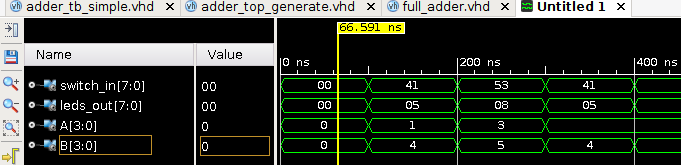
\includegraphics[width=1.2\textwidth]{03-vhdl_modeling/fig/tb_wave.png}
\caption{Окно вейформ сигналов}
\label{tb-wave}
\end{figure}

\item Разобрать текст тесбенча (см. листинг \ref{tb_0}). В строчках 3-4 задается название верхнего VHDL модуля для симуляции. Обратите внимание, что этот модуль не имеет интерфейса. Затем в разделе объявлений архитектуры определяются компонент DUT (наша моделируемая схема) и подключаемые к этому компоненту сигналы. В тестбенче будут заданы последовательности значений, подаваемых на входы схемы DUT. После \emph{begin} сразу идет вставка компонента DUT (строчки 26-29). После чего объявлен всего один процесс, внутри которого генерируются последовательности входных воздействий. В данном случае надо задавать разные слагаемые и смотреть результат суммы в окне вейформ. 
Процесс \emph{stim\_proc} не имеет списка чувствительности, а это значит, что он запуститься сразу (безусловно), как только начнется симуляция. Сразу же сигналам A и B будут присвоены нулевые значения. Далее через каждый 100 ns (с помощью кострукции \emph{wait for 100 ns;}, которая заставляет процесс засыпать на указанное время) значения A и B будут несколько раз изменены. Читателю предлагается проверить в окне вейформ, что сумма остается верной. В конце процесса стоит конструкция \emph{wait;}. Это инструкция бесконечного ожидания, выполнив ее процесс заснет навсегда до конца симуляции. Если бы ее не было, то процесс бы завершился, а потом бы опять сразу начался с самого начала, т.к. его список чувствительности пуст. 

% \begin{Code}
\lstinputlisting[caption=Простая тестбенч, label=tb_0]{02-vhdl_basics/lab2-1/src/adder_tb_simple.vhd}
% \end{Code}

\item Далее читателю предлагается самостоятельно поиграть с тестбенчем, изменяя код генерации входных воздействий. Можно задавать любые времянные промежутки, другие значения слагаемых. Каждый раз после изменения кода, его необходимо компилировать заново. Для этого удобно использовать кнопку \emph{Relaunch}, которая находится прямо над окном вейформ. Если код не менялся, а просто были добавлены новые сигналы на вейформу, то можно не перекомпилировать код, а достаточно просто запустить моделирование с нуля времени с помощью кнопок \emph{Restart} и \emph{Run}, находящихся слева от \emph{Relaunch}. При этом можно обратить внимание, что все нажатия на кнопки дублируются командами в окне \emph{Tcl Console}.  

\end{enumerate}